\chapter{Ocena aplikacji}
\label{cha:ocena}

W tym rozdziale zaprezentowana jest kompleksowa ocena aplikacji \en podzielona
na kilka kluczowych części. Najpierw przedstawione są testy jakościowe, które
polegają na próbie odzwierciedlenia wybranych zjawisk fizycznych przy pomocy
symulatora. Z kolei testy wydajnościowe silników fizycznych w wersji
podstawowej oraz równoległej pokazują zysk jaki dało przeniesienie obliczeń na
kartę graficzną. Na podstawie tych wyników zanalizowana została dostępność
aplikacji dla potencjalnych użytkowników na różnych urządzeniach oraz ich
konfiguracjach.

\section{Modelowanie wybranych zjawisk fizycznych jako testy jakościowe symulatora}

W przypadku aplikacji edukacyjnej jaką jest symulator \en niezwykle istotne
jest aby symulowane zjawiska odzwierciedlały w sposób  wiarygodny
rzeczywistość. Z drugiej strony, aplikacja musi być interaktywna i
działać w czasie rzeczywistym. Dlatego też nie można sobie pozwolić na zbyt
długi czas wykonywania, co zwykle idzie w parze z dokładnymi algorytmami i
obliczeniami. Z tego też powodu zastosowane silniki fizyczne (por. rozdział
\ref{sec:silnikiFizyczne}) balansują pomiędzy poprawnością fizyczną, a
wydajnością. Jest to dopuszczalne, ponieważ symulacja jest zorientowana
wyłącznie na aspekt wizualny.

Z powodu tego kompromisowego podejścia do pełnej dokładności obliczeń niezwykle
istotne były testy aplikacji pod kątem podstawowej poprawności fizycznej. W tym
celu zostały przygotowane przypadki testowe, które miały za zadanie modelować
powszechnie znane zjawiska fizyczne związane z przewodnictwem cieplnym oraz
dynamiką płynów. Poniżej przedstawione są wyniki tych testów.

\subsection{Komórki Bénarda}

Modelowanie komórek Bénarda to jeden z podstawowych testów aplikacji
symulujących dynamikę płynów. Są to komórki konwekcyjne powstające w płynie
podgrzewanym od spodu. Rysunek \ref{fig:physBenard} prezentuje wyniki symulacji
przeprowadzonej przez \en.

\begin{figure}[!h]
\centering
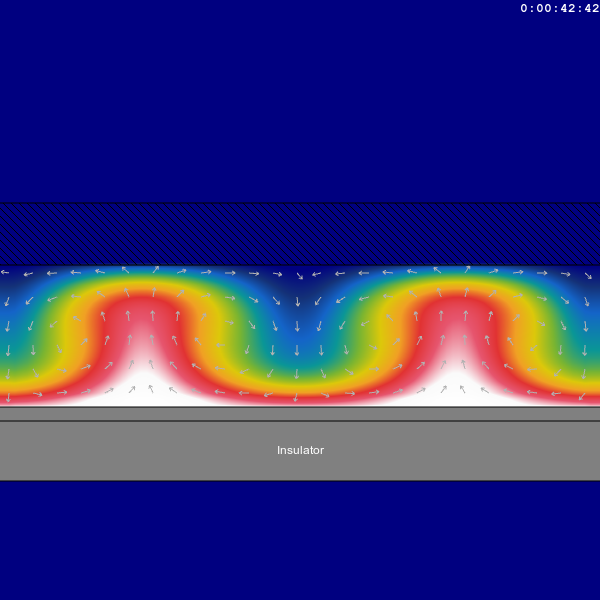
\includegraphics[width=0.8\textwidth]{img/physics/benard}
\caption{Symulacja formowania się komórek Bénarda}
\label{fig:physBenard}
\end{figure}

Wyraźnie widać formowanie się oczekiwanych komórek. Ich układ oraz kształt
stabilizuje się po bardzo krótkim czasie symulacji. Wyniki można uznać za w
pełni satysfakcjonujące.

\subsection{Przepływ laminarny oraz turbulentny}
\label{sec:przeplywyLamTur}

Symulacja przepływów laminarnych oraz turbulentnych to następny test silnika
dynamiki płynów. Rodzaj przepływu, w przypadku gdy jest on zakłócony przez
obecność przeszkody, w głównym stopniu determinuje liczba Reynoldsa. Jest ona
zależna od:

\begin{itemize}
\item lepkości płynu,
\item prędkości przepływu,
\item średnicy przeszkody.
\end{itemize}

W związku z tym został przygotowany przypadek testowy, w którym płyn ma stałą
lepkość, a przeszkody identyczne wymiary. Zmienna jest tylko prędkość przepływu.
Dla mniejszych prędkości oczekiwanym wynikiem był przepływ laminarny, dla
większych przepływ turbulentny. Rysunek \ref{fig:physLaminarTurbulent}
prezentuje wyniki takiej symulacji przeprowadzonej przez \en.

\begin{figure}[!h]
\centering
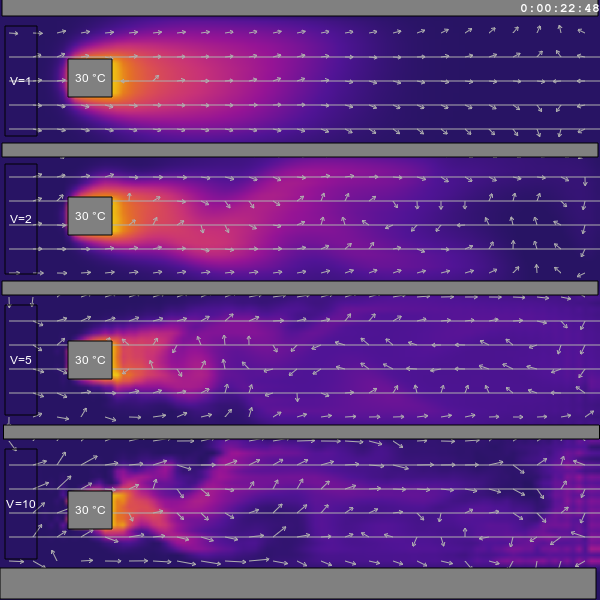
\includegraphics[width=0.8\textwidth]{img/physics/laminarTurbulent}
\caption{Symulacja wpływu liczby Reynoldsa na rodzaj przepływu}
\label{fig:physLaminarTurbulent}
\end{figure}

Rezultaty są zgodne z oczekiwaniami. Wyraźnie widać wpływ liczby Reynoldsa
(determinowanej przez prędkość płynu) na rodzaj przepływu.

\subsection{Ścieżka wirowa von Kármána}

Ścieżka wirowa von Kármána to kolejny doskonały test silnika dynamiki płynów.
Jest to szczególny rodzaj przepływu turbulentnego, który powstaje wyłącznie dla
pewnego zakresu wartości liczby Reyonldsa (por. \ref{sec:przeplywyLamTur}).

W związku z tym został przygotowany przypadek testowy, w którym płyn ma stałą
lepkość oraz prędkość przepływu, natomiast zmienna jest tylko średnica
przeszkody. Zgodnie z powyższymi założeniami powinno być możliwe dobranie
takich średnic przeszkód, aby wiry von Kármána powstały tylko za jedną z nich.
Rysunek \ref{fig:physKarman} prezentuje wyniki takiej symulacji przeprowadzonej
przez \en.

\begin{figure}[!h]
\centering
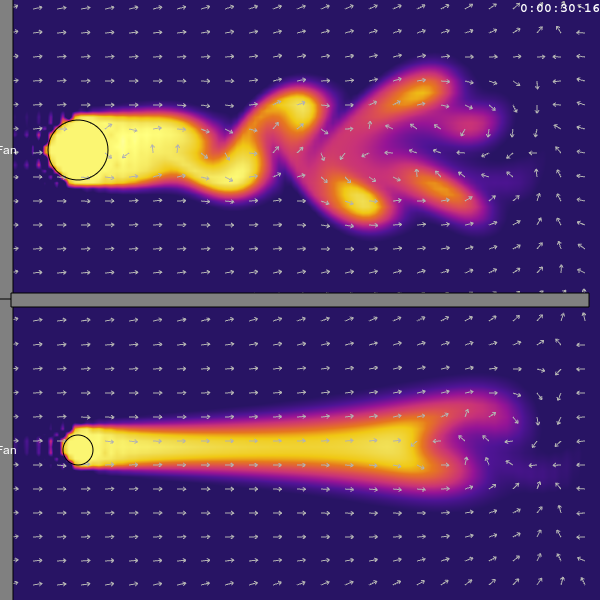
\includegraphics[width=0.8\textwidth]{img/physics/karman}
\caption{Symulacja formowania się wirów Kármána}
\label{fig:physKarman}
\end{figure}

Rezultaty są zgodne z oczekiwaniami. Ścieżka wirowa powstała tylko w warunkach, w których
liczba Reynoldsa była większa.

\subsection{Pojemność cieplna}

Tym razem przypadek testowy dotyczy silnika przewodnictwa cieplnego. Pojemność
cieplna to wielkość fizyczna, która charakteryzuje ilość ciepła jaka jest
niezbędna do zmiany temperatury ciała o jednostkę temperatury. Poprawna
symulacja powinna uwzględniać ten parametr materiałów.

Aby to sprawdzić przygotowany został przypadek testowy, w którym znajdują się
dwa materiały o różnej pojemności cieplnej ogrzewane przez otoczenie. Materiał
o większej pojemności powinien przewodzić ciepło znacznie gorzej niż materiał
o pojemności mniejszej. Wyniki takiego eksperymentu przeprowadzonego przez
symulator \en prezentuje rysunek \ref{fig:heatCapacity}.

\clearpage 

\begin{figure}[!h]
\centering
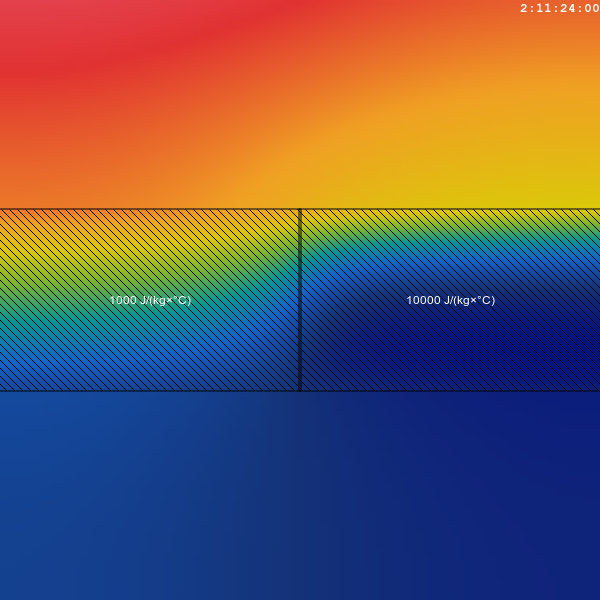
\includegraphics[width=0.8\textwidth]{img/physics/heatCapacity}
\caption{Symulacja wpływu pojemności cieplnej na przewodnictwo cieplne}
\label{fig:heatCapacity}
\end{figure}


Rezultaty po raz kolejny są zgodne z oczekiwaniami. Widać wyraźnie, iż po tym
samym czasie materiał o mniejszej pojemności cieplnej nagrzał się znacznie
bardziej niż materiał o większej pojemności cieplnej.

\subsection{Aspekt edukacyjny}

Ostatni z zaprezentowanych testów jest bardziej złożony. Nie prezentuje on
jednego, konkretnego zjawiska fizycznego jak poprzednie przypadki testowe.
Skupia się on na zaprezentowaniu kompleksowych możliwości symulacji oraz na
aspekcie edukacyjnym.

Przygotowana została scena zawierająca nieszczelnie izolowane pomieszczenie,
będące metaforą mieszkania. Jest ono ogrzewane przez element grzewczy o stałej
mocy. W jego otoczeniu został wymuszony dość mocny przepływ symulujący wiatr.
Miało to na celu pokazanie użytkownikom różnych, potencjalnych dróg ucieczki
ciepła z pomieszczeń mieszkalnych. Rysunek \ref{fig:wind} prezentuje rezultaty
takiej symulacji.

\begin{figure}[!h]
\centering
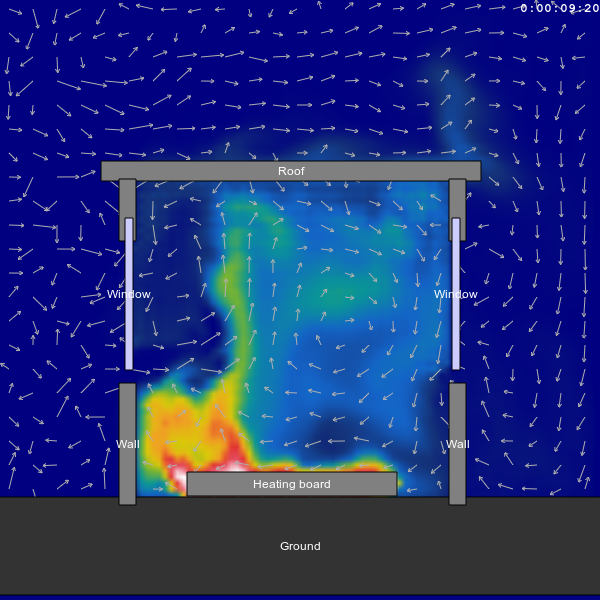
\includegraphics[width=0.8\textwidth]{img/physics/wind}
\caption{Symulacja ucieczki ciepła z pomieszczeń mieszkalnych}
\label{fig:wind}
\end{figure}

Widoczne są dwa wyraźne zjawiska -- utrata ciepła w okolicy nieszczelnych
okien oraz utrata ciepła związana z przewodnictwem cieplnym dachu. Pozwala to
lepiej zrozumieć użytkownikowi wpływ różnych aspektów pomieszczeń mieszkalnych
(takich jak szczelność czy izolacja) na straty ciepła. Może przyczynić się to
do rozsądniejszego i ekonomiczniejszego gospodarowania energią w jego własnym
mieszkaniu lub domu. W dobie szczególnej dbałości o środowisko naturalne jest
to niezwykle cenny i pożądany efekt edukacyjny.

\section{Testy wydajnościowe}
\label{sec:testyWydajnosciowe}

Wydajność jest kluczowym aspektem symulacji ukierunkowanej na cele edukacyjne.
Tylko odpowiednia prędkość symulacji może przyciągnąć uwagę użytkownika i
zachęcić go do dalszej eksploracji zagadnienia.

W celu osiągnięcia zadowalającej wydajności na różnych urządzeniach zastosowano
kilka technik. Podstawową jest świadoma implementacja polegająca na unikaniu
zbędnych, czasochłonnych operacji, wynikająca ze znajomości środowiska
przeglądarki internetowej. Jednak krokiem, który najbardziej przyczynił się do
powstania naprawdę wydajnej aplikacji było przeniesienie obliczeń związanych
z fizyką na procesor karty graficznej.

Niniejszy rozdział przedstawia zyski z zastosowania tej optymalizacji. Omówiona
jest także kwestia wpływu konfiguracji sprzętowej użytkownika oraz związana z
tym ogólna dostępność symulatora dla szerokiego grona odbiorców.

\subsection{Metodologia testów}
\label{sec:metodologiaTestow}

Za wyznacznik wydajności została przyjęta liczba klatek na sekundę animacji,
którą jest w stanie generować działająca aplikacja \en. Jedna klatka animacji
domyślnie składa się z:

\begin{itemize}
\item czterech kroków symulacji, 
\item odświeżenia wizualizacji.
\end{itemize}

Takie też ustawienia zostały zastosowane podczas wszystkich testów.  Aplikacja
wymusza kolejne klatki poprzez użycie metody \ow{setInterval()} z czasem 0.
Powoduje to, iż przeglądarka nie wprowadzi żadnych dodatkowych opóźnień między
klatkami i przejdzie do generowania kolejnej natychmiast, gdy będzie to
możliwe. Nie została użyta zalecana w przypadku aplikacji korzystających z
\ow{WebGL} funkcja \ow{requestAnimationFrame()}, ponieważ wprowadza ona limit
60 klatek na sekundę i koncentruje się na utrzymaniu stałego tempa animacji, a
nie na osiągnięciu maksymalnej wydajności. Zaburzyłoby to w istotny sposób
wiarygodność wyników.

Na potrzeby analizy wydajności zostały przygotowane specjalne przypadki
testowe. Różnią się one między sobą:

\begin{itemize} 
\item układem sceny, 
\item modelowanym zjawiskiem fizycznym,
\item użytymi silnikami fizycznymi:
	\begin{itemize} 
	\item wyłącznie silnik przewodnictwa cieplnego,
	\item silnik przewodnictwa cieplnego oraz silnik dynamiki płynów,
	\end{itemize}
\item rozmiarem siatki symulacyjnej.
\end{itemize}

Tabela \ref{tab:przypTest} prezentuje symboliczne nazwy przypadków testowych
wraz z ich krótką charakterystyką. Skrót HT pochodzi od ang. Heat Transfer i
oznacza, że dany przypadek testowy korzysta z silnika przewodnictwa cieplnego. Z
kolei skrót CDF pochodzi od ang. Computational Fluid Dynamics i oznacza, że dany
przypadek testowy korzysta z silnika dynamiki płynów. Wizualizację symulacji
przypadków testowych prezentują rysunki \ref{fig:ht1}, \ref{fig:ht2},
\ref{fig:cfd1} oraz \ref{fig:cfd2}.

\begin{table}[!h]
\caption{Zestawienie charakterystyki przypadków testowych do pomiaru wydajności}
\centering
\begin{tabular}{|l|c|c|c|l|}
\hline
Nazwa testu & Siatka & HT & CFD & Opis \\ \hline
\textbf{ht1-100} & $100x100$ & \checkmark & $\times$ &
symulacja przewodnictwa cieplnego \\ \hline

\textbf{ht1-512} & $512x512$ & \checkmark & $\times$ &
symulacja przewodnictwa cieplnego \\ \hline

\textbf{ht1-1024} & $1024x1024$ & \checkmark & $\times$ &
symulacja przewodnictwa cieplnego \\ \hline

\textbf{ht2-100} & $100x100$ & \checkmark & $\times$ &
symulacja przewodnictwa cieplnego \\ \hline

\textbf{ht2-512} & $512x512$ & \checkmark & $\times$ &
symulacja przewodnictwa cieplnego \\ \hline

\textbf{ht2-1024} & $1024x1024$ & \checkmark & $\times$ &
symulacja przewodnictwa cieplnego \\ 

\hline \hline 

\textbf{cfd1-100} & $100x100$ & \checkmark & \checkmark &
symulacja dynamiki płynów \\ \hline

\textbf{cfd1-256} & $256x256$ & \checkmark & \checkmark &
symulacja dynamiki płynów \\ \hline

\textbf{cfd2-100} & $100x100$ & \checkmark & \checkmark &
symulacja dynamiki płynów \\ \hline

\textbf{cfd2-256} & $256x256$ & \checkmark & \checkmark &
symulacja dynamiki płynów \\ \hline
\end{tabular}

\label{tab:przypTest}
\end{table}

\begin{figure}[!p]
\begin{minipage}[b]{0.47\linewidth}
\centering
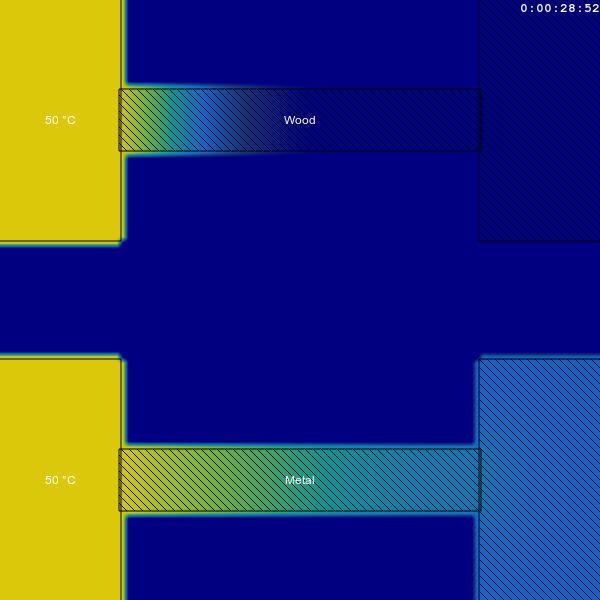
\includegraphics[width=\textwidth]{img/perfCase/ht1}
\caption{Symulacja ht1-100/512/1024}
\label{fig:ht1}
\end{minipage}
\hspace{0.04\linewidth}
\begin{minipage}[b]{0.47\linewidth}
\centering
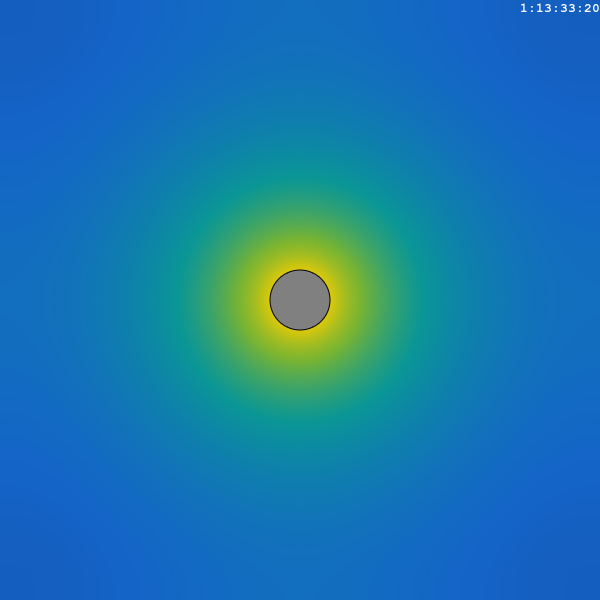
\includegraphics[width=\textwidth]{img/perfCase/ht2}
\caption{Symulacja ht2-100/512/1024}
\label{fig:ht2}
\end{minipage}
\end{figure}
\begin{figure}[!p]
\begin{minipage}[b]{0.47\linewidth}
\centering
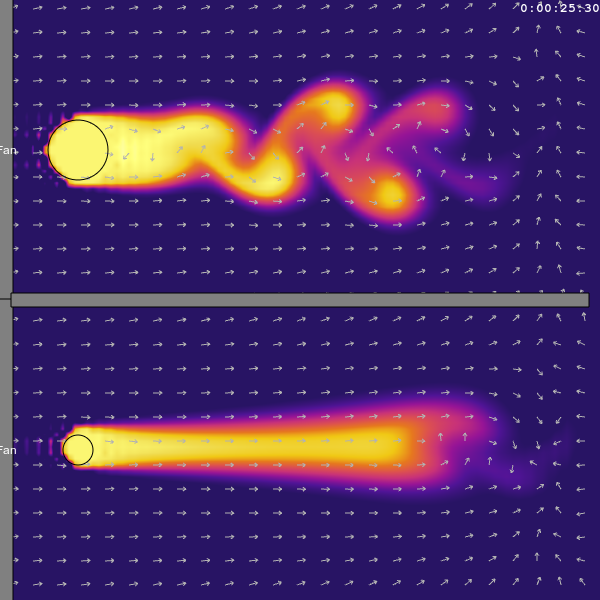
\includegraphics[width=\textwidth]{img/perfCase/cfd1}
\caption{Symulacja cfd1-100/256}
\label{fig:cfd1}
\end{minipage}
\hspace{0.04\linewidth}
\begin{minipage}[b]{0.47\linewidth}
\centering
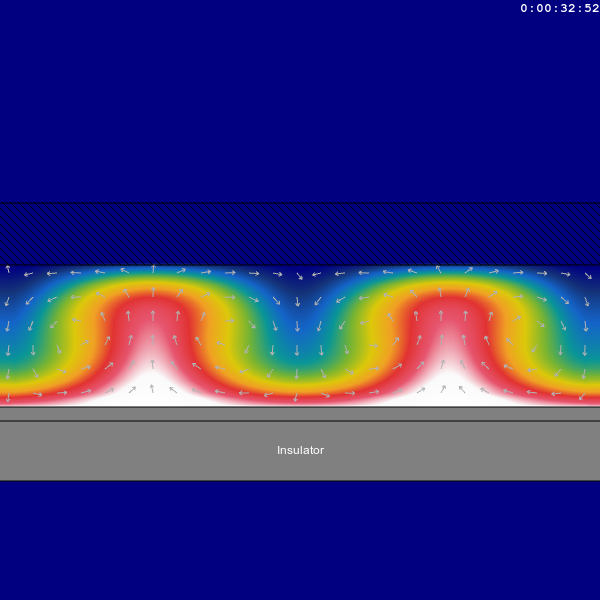
\includegraphics[width=\textwidth]{img/perfCase/cfd2}
\caption{Symulacja cfd2-100/256}
\label{fig:cfd2}
\end{minipage}
\end{figure}

\subsection{Konfiguracje sprzętowe przeznaczone do testów}
\label{sec:konfiguracjaKompow}

Testy zostały przeprowadzone na następujących komputerach:

\begin{itemize}

\item laptop Samsung QX510,
\item laptop Apple MacBook Pro, konfiguracja z roku 2010,
\item laptop Apple MacBook Pro, konfiguracja z roku 2012,
\item komputer stacjonarny, konfiguracja z roku 2008,
\item komputer stacjonarny, konfiguracja z roku 2012.

\end{itemize}

\begin{table}[!h]
\caption{Charakterystyka komputerów testowych}
\centering
\begin{tabular}{|l|l|l|l|}
\hline
Nazwa & Procesor & Karta graficzna & System operacyjny \\ \hline
Samsung QX510 & Intel Core i5 2.66GHz & NVIDIA GT 420M & Ubuntu 12.04 \\ \hline
MacBook Pro 2010 & Intel Core i7 2.66GHz & NVIDIA GT 330M & Mac OS X 10.6.8 \\ \hline
MacBook Pro 2012 & Intel Core i7 2.3GHz & NVIDIA GT 650M & Mac OS X 10.7.4 \\ \hline
Stacjonarny 2008 & Intel Core2Quad 2.5GHz & NVIDIA 9600GT & Windows 7 \\ \hline
Stacjonarny 2012 & Intel i5 3.0GHz & NVIDIA GTX 560 & Windows 7 \\ \hline
\end{tabular}
\label{tab:komputery}
\end{table}

Ich dokładną specyfikację prezentuje tabela \ref{tab:komputery}. Konfiguracje
znacznie różnią się od siebie. W zestawieniu znajdują się zarówno jednostki
mobilne, które cechują się słabszymi, energooszczędnymi podzespołami (w
szczególności dotyczy to kart graficznych), jak i komputery stacjonarne.
Ponadto w każdej z tych grup znajdują się konfiguracje starsze, jak i
najnowsze. Komputery działają pod kontrolą trzech najpopularniejszych systemów
operacyjnych -- Linux (Ubuntu), Mac OS X oraz Windows 7. Pozwoliło to
przeprowadzić przekrojową analizę, która obrazuje rzeczywistą wydajność na
komputerach, które faktycznie mogą posiadać potencjalni użytkownicy.

\subsection{Porównanie wydajności w różnych przeglądarkach internetowych}
\label{sec:przegladarkiWyd}

Aplikacja od samego początku rozwoju była głównie testowana w przeglądarce
Google Chrome, gdyż wyraźnie było widać jej ogromną przewagę w kwestii
wydajności silnika \js. Ponadto wg. najnowszych raportów jest to
najpopularniejsza przeglądarka na świecie, tak więc potencjalnie najwięcej
użytkowników \en będzie z niej korzystać. Raport \cite{BrowserStats} pokazuję,
iż w lipcu 2012 roku z przeglądarki Google Chrome korzystało 42.9\%
użytkowników internetu. Drugie miejsce należało do przeglądarki Mozilla
Firefox z udziałem 33.7\%. Łącznie te dwie przeglądarki posiadają 77.6\%
,,rynku'', dlatego są traktowane priorytetowo. Kolejna popularna przeglądarka
Internet Explorer została wyłączona z testów z powodu niedostępności poza
środowiskiem Windows oraz braku wsparcia dla technologii \ow{WebGL}. Podobnie
Safari, które wspiera \ow{WebGL} jednak działa tylko na systemie operacyjnym
Mac OS. Ostatecznie testy wpływu przeglądarki na wydajność symulacji zostały
przeprowadzone z użyciem następujących aplikacji:

\begin{itemize}
\item Google Chrome v. 22
\item Mozilla Firefox v. 16
\item Opera v. 12.50
\end{itemize}

Użycie różnych konfiguracji sprzętowych powoduje oczywiście zmianę wyników,
jednak względne różnice w wydajności pomiędzy przeglądarkami pozostają bez
zmian. Dlatego też w testach wydajności przeglądarek prezentowane są wyłącznie
wyniki dla laptopa Samsung QX510 (por. tablica \ref{tab:komputery}). Wyniki
dla pozostałych konfiguracji nie wniosłyby nowych oraz wartościowych
informacji.

\subsubsection{Obliczenia fizyczne wykonywane na CPU}

Wyniki pomiarów wpływu przeglądarek na wydajność symulacji w przypadku
obliczeń przeprowadzanych na CPU prezentuje tabela \ref{tab:przegladarki} oraz
wykres \ref{fig:browserPerf}. Wydajność jest przede wszystkim zależna od
rozmiaru siatki. Nietrudno dostrzec ogromną przewagę przeglądarki Google
Chrome w każdym z testowanych przypadków. Jest to efekt zastosowanego w niej
niezwykle wydajnego silnika \ow{JavaScript} o nazwie V8. Opera oraz Mozilla
Firefox posiadają zbliżoną wydajność, jednak Opera jest nieznacznie szybsza.
Warto też zauważyć, iż kiedy obliczenia fizyczne przeprowadzane są na CPU
jedyną przeglądarką, która zapewnia odpowiednią prędkość wykonywania się
symulacji jest Google Chrome.

\begin{table}[!h]
\caption{Wydajność symulacji na CPU w zależności od przeglądarki}
\centering
\begin{tabular}{|l|r|r|r|}
\hline
Test & Google Chrome & Mozilla Firefox & ~~~~~~~Opera \\ \hline
ht1-100 & 45.20 & 11.12 & 11.83 \\ \hline
ht1-512 & 3.24 & 0.45 & 0.98 \\ \hline
ht1-1024 & 0.92 & 0.11 & 0.25 \\ \hline
ht2-100 & 48.04 & 10.73 & 12.05 \\ \hline
ht2-512 & 3.34 & 0.40 & 0.84 \\ \hline
ht2-1024 & 0.89 & 0.11 & 0.22 \\ \hline
\hline
cfd1-100 & 22.25 & 2.51 & 3.84 \\ \hline
cfd1-256 & 4.24 & 0.38 & 0.93 \\ \hline
cfd2-100 & 20.60 & 2.35 & 4.58 \\ \hline
cfd2-256 & 3.71 & 0.30 & 0.73 \\ \hline
\end{tabular}
\label{tab:przegladarki}
\end{table}

\begin{figure}[!h]
\centering
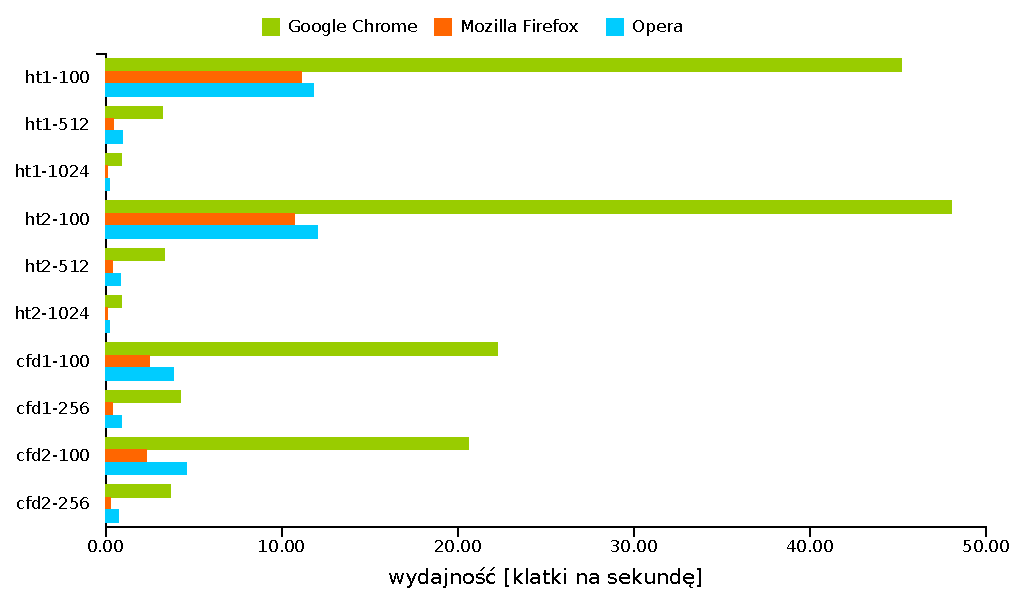
\includegraphics[width=\textwidth]{img/browserPerf}
\caption{Wydajność symulacji na CPU w zależności od przeglądarki}
\label{fig:browserPerf}
\end{figure}

\clearpage

\subsubsection{Obliczenia fizyczne wykonywane na GPU}

W przypadku symulacji, która obliczenia fizyczne przeprowadza na GPU, nie
została przetestowana Opera.  W dniu kiedy testy były przeprowadzane, Opera
oferowała wyłącznie eksperymentalne wsparcie dla technologii \ow{WebGL} i nie
zapewniała dostępu do niezbędnego rozszerzenia \ow{OES\_texture\_float}. Wyniki
pomiarów wpływu pozostałych przeglądarek na wydajność symulacji w przypadku
obliczeń przeprowadzanych na GPU prezentuje tabela \ref{tab:przegladarkiGPU}
oraz wykres \ref{fig:browserPerfGPU}.

\begin{table}[H]
\caption{Wydajność symulacji na GPU w zależności od przeglądarki}
\centering
\begin{tabular}{|l|r|r|}
\hline
Test & Google Chrome & Mozilla Firefox \\ \hline
ht1-100 & 51.57 & 37.33 \\ \hline
ht1-512 & 12.94 & 12.99 \\ \hline
ht1-1024 & 3.73 & 3.64 \\ \hline
ht2-100 & 48.84 & 37.59 \\ \hline
ht2-512 & 12.52 & 12.28 \\ \hline
ht2-1024 & 3.60 & 3.47 \\ \hline
\hline
cfd1-100 & 36.67 & 30.59 \\ \hline
cfd1-256 & 13.47 & 12.35 \\ \hline
cfd2-100 & 33.28 & 31.01 \\ \hline
cfd2-256 & 10.85 & 11.18 \\ \hline
\end{tabular}
\label{tab:przegladarkiGPU}
\end{table}

\begin{figure}[H]
\centering
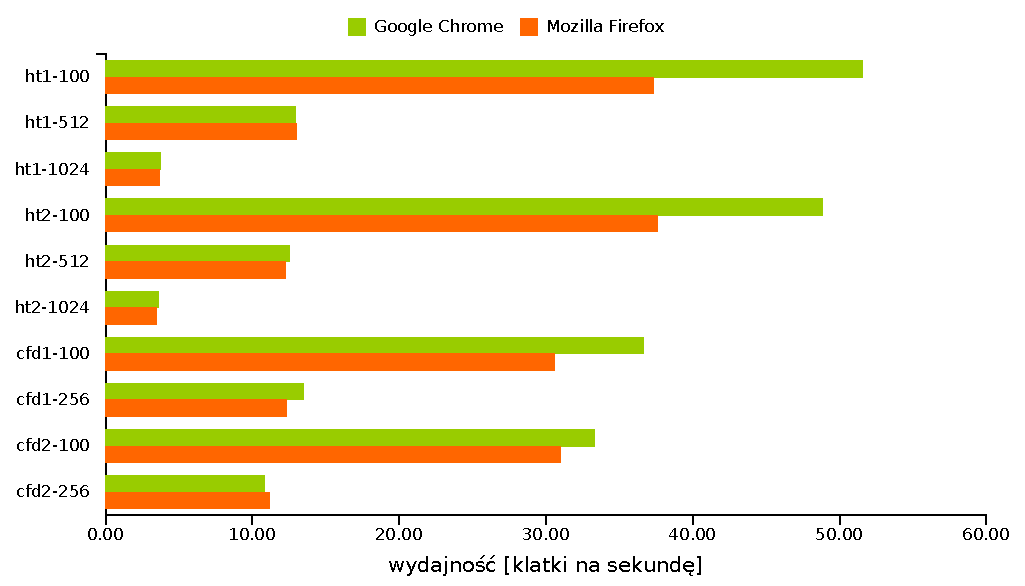
\includegraphics[width=0.9\textwidth]{img/browserPerfGPU}
\caption{Wydajność symulacji na GPU w zależności od przeglądarki}
\label{fig:browserPerfGPU}
\end{figure}

W przypadku obliczeń na GPU sytuacja diametralnie się zmienia. Różnice między
przeglądarkami, tak istotne przy obliczeniach na CPU, stają się znikome.
Wynika to z tego, iż najbardziej obciążające obliczenia przeniesione są na
kartę graficzną i to jej wydajność jest decydująca, a nie wydajność samego
silnika \ow{JavaScript}.  Potwierdza to fakt, iż wraz ze wzrostem wielkości
siatki symulacyjnej różnice między przeglądarkami zanikają. Przewagę Google
Chrome widać wyłącznie dla testów działających na najmniejszych siatkach. Są
to jedyne przypadki, gdzie czas potrzebny na realizacje instrukcji \js
stanowi zauważalny procent czasu wykonywania się całej symulacji.

Innym ważnym wnioskiem jest to, iż użycie technologii \ow{WebGL} pozwala
zniwelować różnice między wydajnością przeglądarek. O ile w przypadku obliczeń
na CPU jedynym rozsądnym środowiskiem wykonywania się symulacji była
przeglądarka Google Chrome, to przy zastosowaniu \ow{WebGL} możliwe staje się
również użycie Mozilli Firefox oraz każdej innej przeglądarki, która wspiera
\ow{WebGL} (np. Safari czy też w niedalekiej przyszłości także Opery).

\subsection{Analiza zysku wydajności wynikającego z przeniesienia obliczeń na GPU}
\label{sec:analizaGPUCPU}

Kluczową optymalizacją wydajności symulatora \en było przeniesienie obliczeń
związanych z fizyką na procesor karty graficznej przy wykorzystaniu technologii
\ow{WebGL}. Szczegóły implementacyjne oraz najważniejsze zagadnienie z tym
związane porusza rozdział \ref{cha:oblGPU}. Niniejsza sekcja przedstawia i
analizuje efekty jakie przyniosła ta optymalizacja.

\begin{description}

\item[Metodologię testów] definiuje podrozdział \ref{sec:metodologiaTestow}.

\item[Konfiguracje sprzętowe] użyte podczas testów przybliża podrozdział
\ref{sec:konfiguracjaKompow}.

\item[Wybór przeglądarki internetowej] do testów jest niezwykle istotnym
czynnikiem, który w największym stopniu determinuje ocenę optymalizacji. Wynika
to z bardzo dużych różnic między wydajnością interpreterów \ow{JavaScript} w
różnych przeglądarkach (por. podrozdział \ref{sec:przegladarkiWyd}). Oczywistym
jest, że przeglądarka o niższej wydajności silnika \ow{JavaScript} zanotuje
znacznie większe przyspieszenie niż przeglądarka o silniku bardzo wydajnym.
Dlatego też do testów została użyta \textbf{najwydajniejsza} z dostępnych
przeglądarek -- Google Chrome. Dzięki temu testy przedstawiają
\textbf{minimalne, pesymistyczne} oczekiwane przyspieszenie związane z
przeniesieniem obliczeń  na GPU. Jednocześnie należy podkreślić, iż na mniej
wydajnych przeglądarkach optymalizacja przynosi jeszcze więcej korzyści i
często staje się niezbędna aby symulację można było określić mianem
interaktywnej.

\end{description}

Wyniki testów na różnych komputerach przestawiają tabele od
\ref{tab:wynikiWebGL_first} do \ref{tab:wynikiWebGL_last}. Zgodnie z przyjętą
metodologią miarą wydajności jest liczba klatek na sekundę jaką jest w stanie
wygenerować przeglądarka podczas działania symulacji. Kolumna \ow{CPU}
prezentuje wydajność symulacji na procesorze głównym, a kolumna \ow{GPU} na
procesorze karty graficznej. Z kolei kolumna \ow{GPU/CPU} prezentuje stosunek
wartości z kolumny \ow{GPU} do wartości z kolumny \ow{CPU}. Jest to pomocniczy
współczynnik, który bardzo dobrze charakteryzuje i wizualizuje zysk z
optymalizacji.

\begin{table}[!htp]
\caption{Wydajność symulacji na CPU oraz GPU -- Google Chrome, laptop Samsung QX510}
\centering
\begin{tabular}{|l|r|r|>{\bfseries}c|}
\hline
\cellcolor{t} Test & \cellcolor{cpu} CPU & \cellcolor{gpu} GPU & \cellcolor{gc} GPU/CPU \\ \hline
ht1-100 & 41.98 & 68.73 & 1.64 \\ \hline
ht1-512 & 3.15 & 12.30 & 3.90 \\ \hline
ht1-1024 & 0.71 & 3.58 & 5.04 \\ \hline
ht2-100 & 51.37 & 62.36 & 1.21 \\ \hline
ht2-512 & 2.86 & 12.61 & 4.41 \\ \hline
ht2-1024 & 0.80 & 3.75 & 4.69 \\ \hline
\hline
cfd1-100 & 18.84 & 43.76 & 2.32 \\ \hline
cfd1-256 & 3.88 & 13.56 & 3.49 \\ \hline
cfd2-100 & 20.60 & 43.28 & 1.62 \\ \hline
cfd2-256 & 3.71 & 10.85 & 2.92 \\ \hline
\end{tabular}
\label{tab:wynikiWebGL_first}
\end{table}

\begin{table}[!htp]
\caption{Wydajność symulacji na CPU oraz GPU -- Google Chrome, laptop Apple MacBook Pro 2010}
\centering
\begin{tabular}{|l|r|r|>{\bfseries}c|}
\hline
\cellcolor{t} Test & \cellcolor{cpu} CPU & \cellcolor{gpu} GPU & \cellcolor{gc} GPU/CPU \\ \hline
ht1-100 & 43.10 & 92.60 & 2.15 \\ \hline
ht1-512 & 3.20 & 15.50 & 4.84 \\ \hline
ht1-1024 & 0.91 & 4.90 & 5.38 \\ \hline
ht2-100 & 43.70 & 92.10 & 2.11 \\ \hline
ht2-512 & 2.91 & 15.50 & 5.33 \\ \hline
ht2-1024 & 0.73 & 4.55 & 6.23 \\ \hline
\hline
cfd1-100 & 21.00 & 55.10 & 2.62 \\ \hline
cfd1-256 & 2.30 & 14.60 & 6.35 \\ \hline
cfd2-100 & 8.00 & 48.00 & 6.00 \\ \hline
cfd2-256 & 1.70 & 12.20 & 7.18 \\ \hline
\end{tabular}
\label{tab:wynikiWebGL_2}
\end{table}

\begin{table}[!htp]
\caption{Wydajność symulacji na CPU oraz GPU -- Google Chrome, laptop Apple MacBook Pro 2012}
\centering
\begin{tabular}{|l|r|r|>{\bfseries}c|}
\hline
\cellcolor{t} Test & \cellcolor{cpu} CPU & \cellcolor{gpu} GPU & \cellcolor{gc} GPU/CPU \\ \hline
ht1-100 & 57.00 & 116.00 & 2.04 \\ \hline
ht1-512 & 4.10 & 53.60 & 13.07 \\ \hline
ht1-1024 & 1.10 & 14.90 & 13.55 \\ \hline
ht2-100 & 79.80 & 118.80 & 1.49 \\ \hline
ht2-512 & 4.60 & 50.30 & 10.93 \\ \hline
ht2-1024 & 0.96 & 14.20 & 14.79 \\ \hline
\hline
cfd1-100 & 17.10 & 101.00 & 5.91 \\ \hline
cfd1-256 & 2.80 & 36.60 & 13.07 \\ \hline
cfd2-100 & 19.90 & 93.00 & 4.67 \\ \hline
cfd2-256 & 2.80 & 36.60 & 13.07 \\ \hline
\end{tabular}
\label{tab:wynikiWebGL_3}
\end{table}

\begin{table}[!htp]
\caption{Wydajność symulacji na CPU oraz GPU -- Google Chrome, komputer stacjonarny 2008}
\centering
\begin{tabular}{|l|r|r|>{\bfseries}c|}
\hline
\cellcolor{t} Test & \cellcolor{cpu} CPU & \cellcolor{gpu} GPU & \cellcolor{gc} GPU/CPU \\ \hline
ht1-100 & 35.00 & 78.00 & 2.23 \\ \hline
ht1-512 & 2.50 & 37.00 & 14.80 \\ \hline
ht1-1024 & 0.69 & 9.00 & 13.04 \\ \hline
ht2-100 & 39.00 & 83.00 & 2.13 \\ \hline
ht2-512 & 2.25 & 37.00 & 16.44 \\ \hline
ht2-1024 & 0.65 & 10.60 & 16.31 \\ \hline
\hline
cfd1-100 & 16.55 & 64.10 & 3.87 \\ \hline
cfd1-256 & 2.50 & 30.00 & 12.00 \\ \hline
cfd2-100 & 12.80 & 65.20 & 5.09 \\ \hline
cfd2-256 & 2.15 & 26.30 & 12.23 \\ \hline
\end{tabular}
\label{tab:wynikiWebGL_4}
\end{table}

\clearpage

\begin{table}[!htp]
\caption{Wydajność symulacji na CPU oraz GPU -- Google Chrome, komputer stacjonarny 2012}
\centering
\begin{tabular}{|l|r|r|>{\bfseries}c|}
\hline
\cellcolor{t} Test & \cellcolor{cpu} CPU & \cellcolor{gpu} GPU & \cellcolor{gc} GPU/CPU \\ \hline
ht1-100 & 65.00 & 149.00 & 2.29 \\ \hline
ht1-512 & 4.50 & 67.00 & 14.89 \\ \hline
ht1-1024 & 1.25 & 21.00 & 16.80 \\ \hline
ht2-100 & 79.00 & 149.00 & 1.89 \\ \hline
ht2-512 & 5.20 & 69.00 & 13.27 \\ \hline
ht2-1024 & 1.20 & 22.00 & 18.33 \\ \hline
\hline
cfd1-100 & 30.45 & 140.00 & 4.60 \\ \hline
cfd1-256 & 5.80 & 58.00 & 10.00 \\ \hline
cfd2-100 & 21.60 & 143.00 & 6.62 \\ \hline
cfd2-256 & 4.65 & 48.00 & 10.32 \\ \hline
\end{tabular}
\label{tab:wynikiWebGL_last}
\end{table}

Bardzo wyraźna jest zależność wyników od konfiguracji sprzętowej. Wyniki można
rozpatrywać pod kątem bezwzględnych wartości liczby klatek na sekundę oraz pod
kątem zysku z optymalizacji polegającej na przeniesieniu obliczeń na GPU
(reprezentowanego przez współczynnik GPU/CPU). W przypadku wartości
bezwzględnych oczywistym jest, iż najszybsza powinna okazać się najmocniejsza
jednostka w zestawieniu. Powyższe wyniki to potwierdzają -- zdecydowanie
najszybszy okazał się komputer stacjonarny z roku 2012, co znajduje
uzasadnienie w jego parametrach.

W przypadku znacznie bardziej interesującego parametru jakim jest stosunek
wydajności GPU do CPU, można zauważyć dwie grupy charakteryzujące się dużymi
różnicami w wynikach. Zdecydowanie większy zysk z przeniesienia obliczeń na
GPU odnotowują oba komputery stacjonarne oraz laptop Apple MacBook z roku
2012. Pozostałe dwa laptopy prezentują trochę mniej imponujące rezultaty tej
optymalizacji. Tłumaczy to przede wszystkim specyfikacja kart graficznych oraz
ich odniesienie do mocy procesora danej konfiguracji. Dwie jednostki, które
osiągają najmniejszy zysk, posiadają stosunkowo wydajne procesory, natomiast
karty graficzne są zdecydowanie nastawione na energooszczędność, a nie
maksymalną wydajność. Ponadto w obecnych czasach kolejne modele kart
graficznych pojawiające się rynku przynoszą znacznie większe zmiany w mocy
obliczeniowej niż kolejne modele procesorów głównych. Dlatego też nowsze
karty graficzne w zestawieniu prezentują znacznie bardziej imponujące
rezultaty.

Powyższą obserwację można uogólnić, stwierdzając iż komputery nowocześniejsze,
o większej mocy obliczeniowej, korzystają ze zrównoleglenia obliczeń znacznie
bardziej niż komputery mniej wydajne i starsze. Jest to obiecująca tendencja,
gdyż prognozuje coraz większe korzyści płynące z przenoszenia obliczeń
ogólnego zastosowania na procesory kart graficznych.

Zdecydowanie największy wpływ na przyrost wydajność podczas obliczeń
równoległych ma rozmiar siatki symulacyjnej. Relacje współczynnika GPU/CPU oraz
rozmiaru siatki prezentuje tabela \ref{tab:gpucpu} oraz odpowiadający jej wykres
\ref{fig:gpucpu}. Dane uśredniono z testów na wszystkich pięciu konfiguracjach
sprzętowych.

\begin{table}[!htp]
\caption{Stosunek wydajności obliczeń na GPU do CPU w zależności od rozmiaru
siatki symulacyjnej}
\centering
\begin{tabular}{|l|>{\bfseries}c|}
\hline
\cellcolor{t} Siatka & \cellcolor{gc} GPU/CPU \\ \hline
100x100 & 3.12 \\ \hline
256x256	& 9.06 \\ \hline
512x512	& 10.19 \\ \hline
1024x1024 & 11.42 \\ \hline
\end{tabular}
\label{tab:gpucpu}
\end{table}

\begin{figure}[!h]
\centering
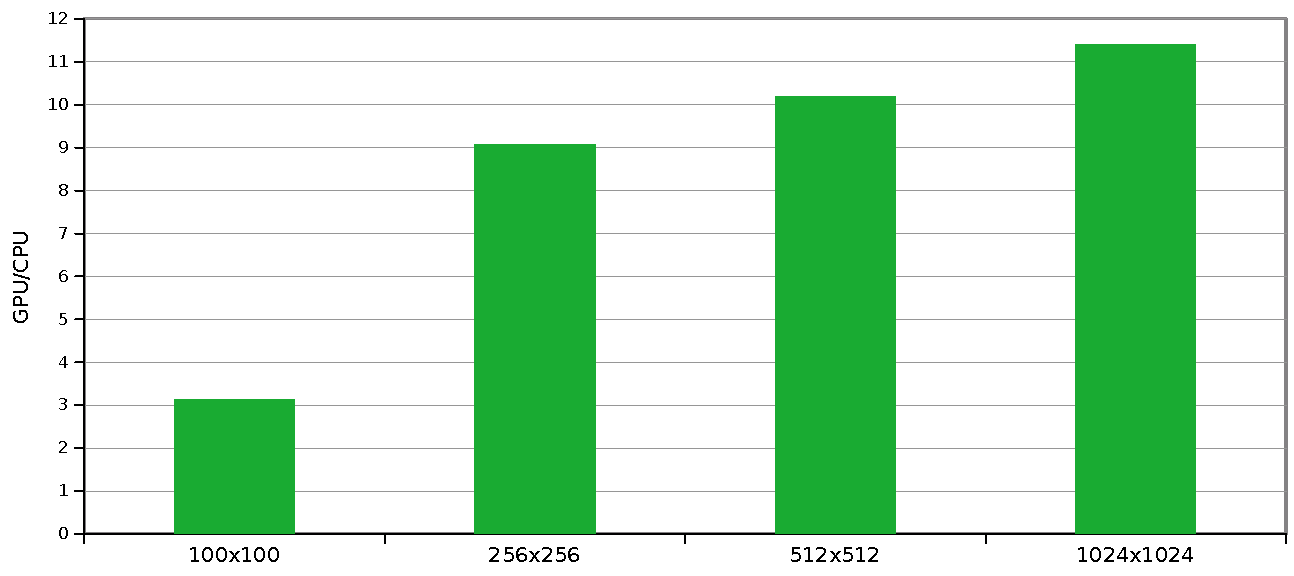
\includegraphics[width=\textwidth]{img/gpucpu}
\caption{Stosunek wydajności obliczeń na GPU do CPU w zależności od rozmiaru
siatki symulacyjnej}
\label{fig:gpucpu}
\end{figure}

Wyniki potwierdzają wartość zastosowanej optymalizacji. Już dla najmniejszej
siatki średni wzrost wydajności jest ponad \textbf{trzykrotny}. Dla większych
siatek wydajność jest średnio \textbf{dziesięć razy większa} niż podczas
obliczeń na CPU.

Odpowiednio gęsta siatka pokazuje potencjał jednostek graficznych. Ponadto
wzrost zysku z optymalizacji wraz ze wzrostem rozmiaru siatki wiążę się też
zapewne z niwelowaniem znaczenia instrukcji w języku \ow{JavaScript} wspólnych
dla wersji zarówno sekwencyjnej jak i równoległej. Gdy rozmiar siatki jest
odpowiednio duży, procent czasu poświęcony na wykonywanie tych instrukcje staje
się pomijalnie mały.

Warto też przypomnieć, że zgodnie z przyjętymi założeniami są to wyniki dla
przeglądarki Google Chrome, która posiada najszybszy silnik \js, a więc
\textbf{najmniej korzystny} do testowania zysków z przeniesienia obliczeń na
GPU. Używając przeglądarki Mozilla Firefox można zaobserwować
\textbf{dwunastokrotny} wzrost wydajności już dla najmniejszych siatek
symulacyjnych. Natomiast użycie większych siatek owocuje ponad
\textbf{trzydziestokrotnym} wzrostem wydajności. Te wartości można obliczyć
korzystając z tabel \ref{tab:przegladarki} oraz \ref{tab:przegladarkiGPU}
znajdujących się w sekcji analizującej wydajność poszczególnych przeglądarek.

\subsection{Wpływ przeniesienia obliczeń na GPU na jakość symulacji}

Oczywiście zrównoleglenie symulacji przekłada się na jej szybsze wykonywanie.
Dokładne wyniki przedstawia poprzednia sekcja \ref{sec:analizaGPUCPU}. W
kontekście aplikacji edukacyjnej jest to bardzo ważne -- symulator staje się
bardziej ,,interaktywny'', a oczekiwane rezultaty widać dużo szybciej.
Doświadczenia i analizy pokazują, że zbyt wolne działanie aplikacji bardzo
często skutkuje szybkim zniechęceniem i znużeniem użytkownika.

Dzięki przeniesieniu obliczeń na GPU, symulacja przyspieszyła około trzykrotnie
już dla siatek 100x100. Często tylko zastosowanie tej optymalizacji pozwala, aby
animacja była odtwarzana z prędkością większą niż 25--30 klatek na sekundę. Jest
to graniczna wartość, dla której ludzkie oko interpretuje animację jako płynną.
Dlatego też zysk z optymalizacji jest nie do przecenienia.

Użycie większej siatki symulacyjnej skutkuje jeszcze większym wzrostem
wydajności podczas obliczeń równoległych. Wydawać by się mogło, iż większa
siatka powinna przynieść automatycznie lepszą jakość symulacji. Jednak przy
zastosowanych algorytmach fizycznych większa siatka wprowadza też pewne problemy
-- trudniej jest symulować wybrane zjawiska fizyczne. Potrzebne jest znacznie
dokładniejsze rozwiązywanie układów równań liniowych (czyli w praktyce wykonanie
większej liczby kroków w metodzie relaksacyjnej), co powoduje zwielokrotnienie
czasu potrzebnego na obliczenia. Efekt ten przedstawiają rysunki
\ref{fig:relaxGPU1} oraz \ref{fig:relaxGPU2}. Przy obecnej wydajności procesorów
głównych oraz graficznych, używanie gęstych siatek symulacji staje się niestety
niepraktyczne. Ponadto minimalnie poprawiony efekt wizualny nie jest warty tak
znacznego spadku wydajności. Dlatego też większość przykładów w finalnej wersji
aplikacji korzysta z siatek 100x100. Taki rozmiar zapewnia dobrą jakość wizualną
i merytoryczną symulacji, a dzięki przeniesieniu obliczeń na GPU również
doskonałą płynność działania.

\begin{figure}[!h]
\centering
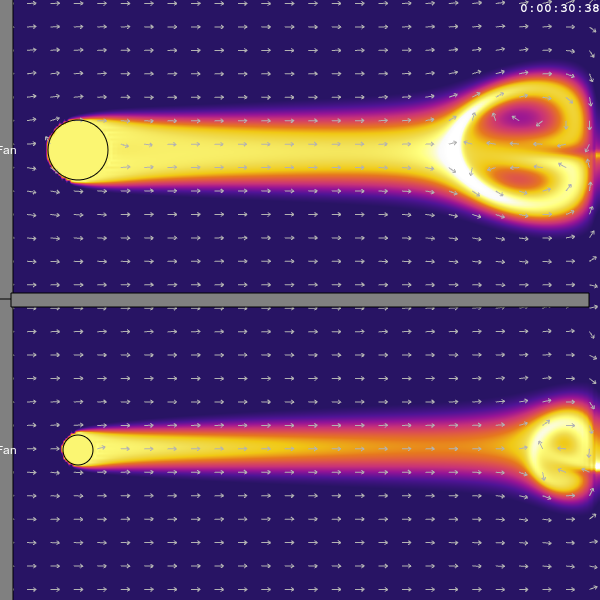
\includegraphics[width=0.6\textwidth]{img/relaxGPU1}
\caption{Niewłaściwie formowanie się ścieżki wirowej von Kármána -- obliczenia na
GPU, siatka 256x256, 10 kroków relaksacji}
\label{fig:relaxGPU1}
\end{figure}

\begin{figure}[!h]
\centering
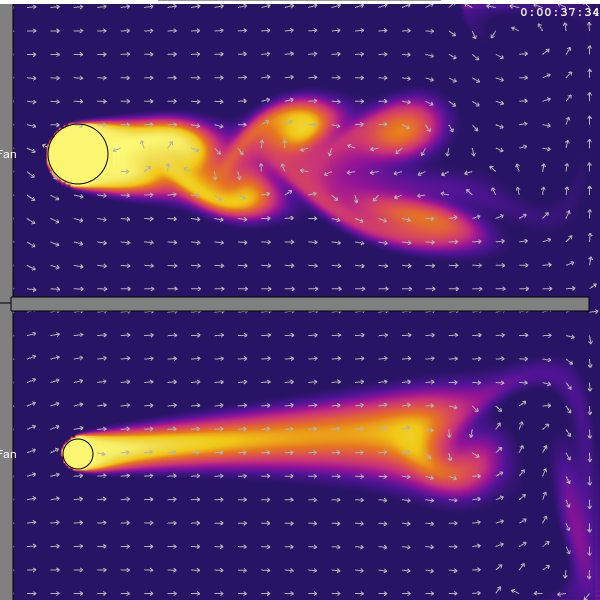
\includegraphics[width=0.6\textwidth]{img/relaxGPU2}
\caption{Właściwe formowanie się ścieżki wirowej von Kármána -- obliczenia na GPU,
siatka 256x256, 60 kroków relaksacji}
\label{fig:relaxGPU2}
\end{figure}

\clearpage

\section{Ocena dostępności aplikacji dla potencjalnych użytkowników}

Symulator \en do działania wymaga wyłącznie przeglądarki internetowej. W
dzisiejszych czasach jest to standardowa aplikacja znajdująca się na prawie
każdym komputerze. Do uruchomienia symulatora \en nie jest wymagana żadna
instalacja zewnętrznych bibliotek, rozszerzeń, a więc nie są też wymagane
uprawnienia administratora. Potencjalnemu użytkownikowi wystarczy
komputer średniej klasy z zainstalowaną przeglądarką internetową oraz dostępem
do internetu. Biorąc pod uwagę możliwości aplikacji, są to niewątpliwie niskie
wymagania.

Wpływ posiadanej konfiguracji sprzętowej i oprogramowania na działanie
symulatora jest istotny. Gdy nie jest możliwe korzystanie z akceleracji na
karcie graficznej to wydajność silnika \ow{JavaScript} zastosowanego w
przeglądarce internetowe ma decydujące znacznie. Testy przedstawia sekcja
\ref{sec:przegladarkiWyd}. Najlepszym wyborem w tym momencie jest przeglądarka
Google Chrome, jednak w związku z dynamicznym rozwojem wszystkich wiodących
przeglądarek sytuacja ta może się zmienić w niedalekiej przyszłości.

Problem zależności od konkretnej przeglądarki likwiduje przeniesienie
obliczeń na kartę graficzną. Interpreter \ow{JavaScript} traci na znaczeniu,
jednak wymagane jest wsparcie przeglądarki dla technologii \ow{WebGL}. W tym
momencie zapewnia je Google Chrome, Mozilla Firefox, Safari oraz Opera (jeszcze
w fazie eksperymentalnej). Czyli przeglądarki, które posiadają zdecydowaną
większość rynku. Ponadto wsparcie dla \ow{WebGL} w niedalekiej przyszłości
powinna zapewniać każda, licząca się przeglądarka internetowa.

Dzięki użyciu tej optymalizacji ciężar obliczeń spada na kartę graficzną. Nawet
niewydajne, energooszczędne karty graficzne przeznaczone dla laptopów radzą
sobie z tym zdaniem doskonale. Dlatego też ograniczenia sprzętowe nie powinny
stanowić problemu dla użytkownika. Uśredniając zgromadzone wyniki testów (por.
sekcja \ref{sec:analizaGPUCPU}), karty graficzne osiągnęły od trzech do
dziesięciu razy lepszą wydajność niż procesory główne i zapewniły doskonałą
płynność symulacji.

